\documentclass[tikz, border=10pt]{standalone}
\usetikzlibrary{arrows}

\begin{document}

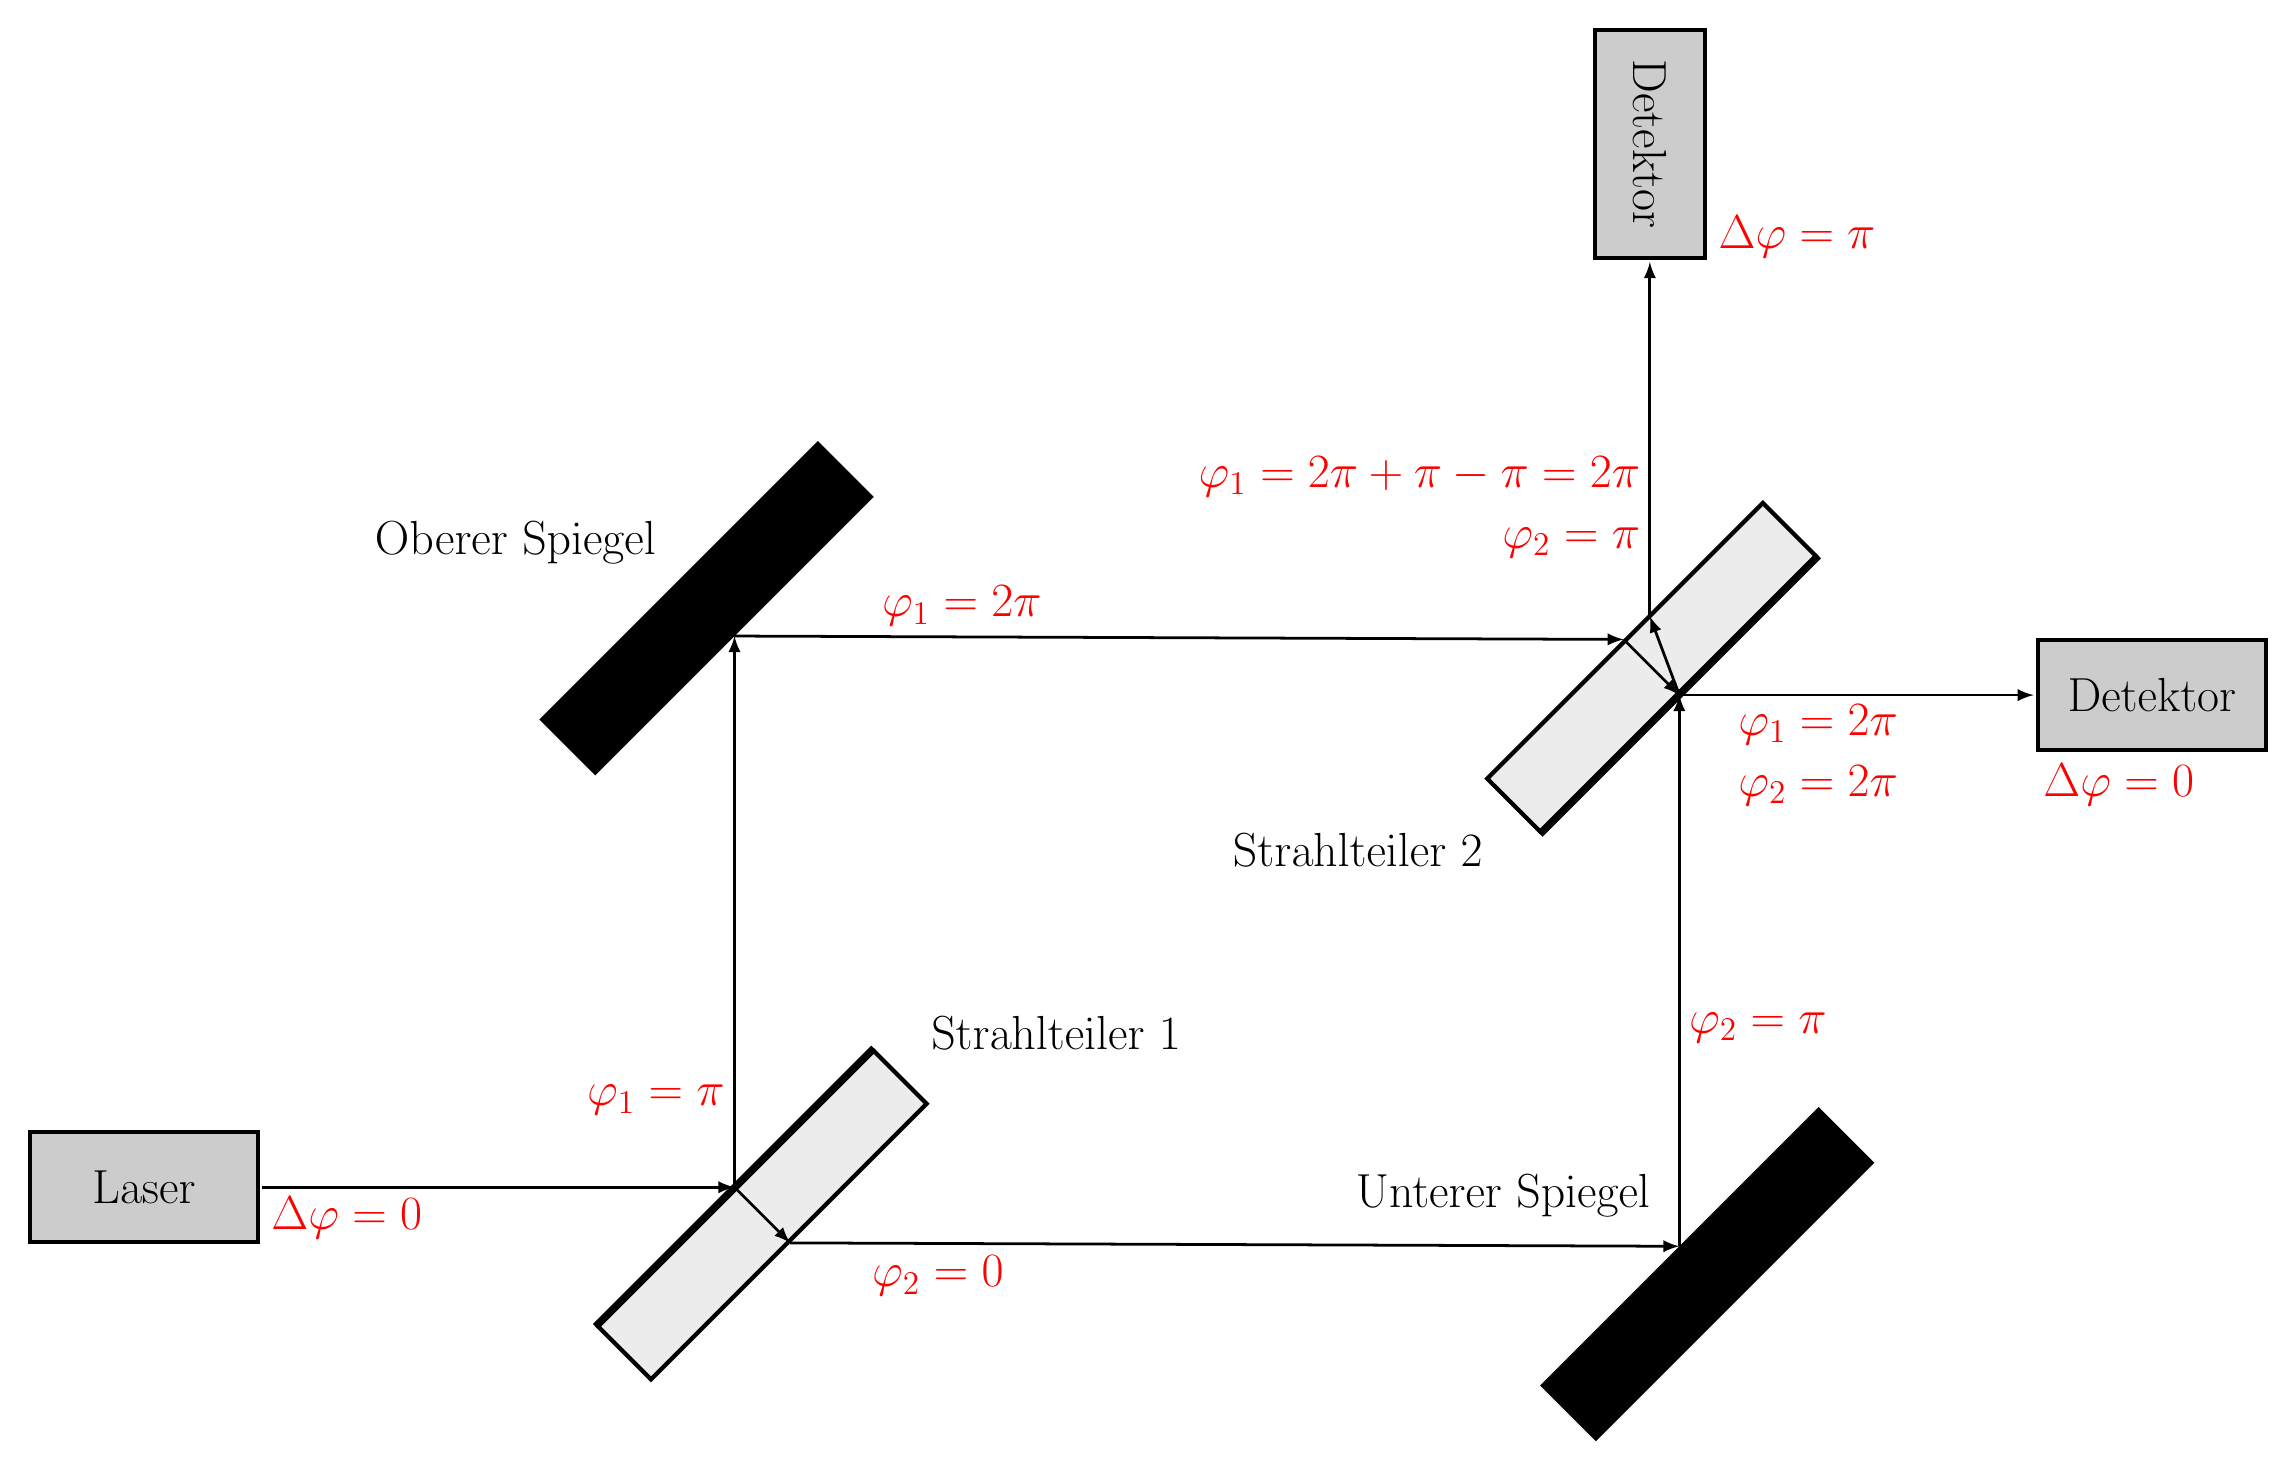
\begin{tikzpicture}

    % --- Grundeinstellungen für Styles ---
    % Definition von Styles macht den Code wartbarer und kürzer
    \tikzset{
        component/.style={draw, line width=1.5pt, minimum width=2.9cm, minimum height=1.4cm, font=\LARGE, align=center},
        laser/.style={component, fill=gray!40},
        detector/.style={component, fill=gray!40},
        splitter/.style={component, fill=gray!15, minimum width=4.95cm, minimum height=0.95cm, rotate=45},
        mirror/.style={component, fill=black, minimum width=4.95cm, minimum height=0.95cm, rotate=45},
        mathlabel/.style={text=red, font=\LARGE, align=left} % Rot, groß, linksbündig
    }

    % --- 1. Optische Komponenten ---
    
    % Laser
    \node[laser] at (5.5, 5.25) {Laser};

    % Strahlteiler 1 (Grau, gedreht)
    \node[splitter] at (13.354, 4.896) {};
    
    % Spiegel Unten (Schwarz, gedreht)
    \node[mirror] at (25.354, 4.146) {};

    % Strahlteiler 2 (Grau, gedreht)
    \node[splitter] at (24.646, 11.854) {};

    % Spiegel Oben (Schwarz, gedreht)
    \node[mirror] at (12.646, 12.604) {};

    % Detektoren
    \node[detector] at (31, 11.5) {Detektor};
    \node[detector, rotate=-90] at (24.625, 18.5) {Detektor};

    % Verstärkungslinien in den Strahlteilern (optische Kennzeichnung)
    \draw[line width=2.5pt] (11.232, 3.482) -- (14.768, 7.018);
    \draw[line width=2.5pt] (23.232, 9.732) -- (26.768, 13.268);


    % --- 2. Lichtwege (Pfeile) ---
    % -latex sorgt für schöne Pfeilspitzen
    \draw[-latex, line width=1pt] (7, 5.25) -- (13, 5.25);
    \draw[-latex, line width=1pt] (13, 5.25) -- (13.707, 4.543);
    \draw[-latex, line width=1pt] (13, 5.25) -- (13, 12.25);
    \draw[-latex, line width=1pt] (13.707, 4.543) -- (25, 4.5);
    \draw[-latex, line width=1pt] (25, 4.5) -- (25, 11.5);
    \draw[-latex, line width=1pt] (13, 12.25) -- (24.293, 12.207);
    \draw[-latex, line width=1pt] (24.293, 12.207) -- (25, 11.5);
    \draw[-latex, line width=1pt] (25, 11.5) -- (24.625, 12.5);
    \draw[-latex, line width=1pt] (24.625, 12.5) -- (24.625, 17);
    \draw[-latex, line width=1pt] (25, 11.5) -- (29.5, 11.5);


    % --- 3. Beschriftungen (Schwarz) ---
    % font=\LARGE sorgt für konsistente Größe ohne manuelles Setzen im Text
    
    \node[font=\LARGE, anchor=south west] at (15.375, 6.875) {Strahlteiler 1};
    \node[font=\LARGE, anchor=north east] at (22.625, 9.875) {Strahlteiler 2};
    \node[font=\LARGE, anchor=south east] at (24.75, 4.75) {Unterer Spiegel};
    
    % Hier war im Original ein 'text width', das zu Problemen führte. Entfernt.
    \node[font=\LARGE, anchor=north east, align=right] at (12.125, 13.836) {Oberer Spiegel};


    % --- 4. Mathematische Beschriftungen (Rot) ---
    % mathlabel style enthält bereits: text=red, font=\LARGE
    % Formeln sind in $...$ eingeschlossen für korrekten Satz

    \node[mathlabel, anchor=north west] at (6.996, 5.25) {$\Delta\varphi=0$};

    \node[mathlabel, anchor=east] at (13, 6.355) {$\varphi_1=\pi$};

    \node[mathlabel, anchor=south west] at (14.75, 12.25) {$\varphi_1=2\pi$};

    \node[mathlabel, anchor=north west] at (14.625, 4.5) {$\varphi_2=0$};

    \node[mathlabel, anchor=north west] at (25.625, 11.5) {$\varphi_1=2\pi$ \\ $\varphi_2=2\pi$};

    \node[mathlabel, anchor=north west] at (29.5, 10.75) {$\Delta\varphi=0$};

    % --- Der kritische Knoten ---
    % Hier wurde align=right gesetzt und text width entfernt, damit die Formel passt.
    % Das Unicode En-Dash (–) wurde durch ein echtes Minus (-) ersetzt.
    \node[mathlabel, align=right, anchor=south east] at (24.625, 13.125) {$\varphi_1 = 2\pi + \pi - \pi = 2\pi$ \\ $\varphi_2 = \pi$};

    \node[mathlabel, anchor=north west] at (25.375, 17.711) {$\Delta\varphi=\pi$};

    \node[mathlabel, anchor=north west] at (25, 7.586) {$\varphi_2=\pi$};

\end{tikzpicture}

\end{document}